%%%%%%%%%%%%%%%%%%%%%%%%%%%%%%%%%%%%%%%%%%%%%%%%%%%%%%%%%%%%%%%%%%%%%%%%%%%%%%%%
%2345678901234567890123456789012345678901234567890123456789012345678901234567890
%        1         2         3         4         5         6         7         8

\documentclass[letterpaper, 9 pt, conference]{ieeeconf}  % Comment this line out
                                                          % if you need a4paper
%\documentclass[a4paper, 10pt, conference]{ieeeconf}      % Use this line for a4
                                                          % paper

\IEEEoverridecommandlockouts                              % This command is only
                                                          % needed if you want to
                                                          % use the \thanks command
\overrideIEEEmargins

\usepackage[english]{babel}
\usepackage[utf8]{inputenc}
\usepackage{amsmath}
\usepackage{graphicx}
\usepackage[colorinlistoftodos]{todonotes}
\usepackage{caption}
\usepackage{subcaption}

\title{\LARGE \bf
Improving Automatic Whiteout++ through Zonal Division of Keyboard
}

\author{Team 3}
%\author{Anurag Kyal, Luke Tornquist, Vinay Kola, and Yuan Ma}

\begin{document}

\maketitle
\thispagestyle{empty}
\pagestyle{empty}
\nocite{*} % Show all Bib-entries

\section{Problem Description}
Mini-QWERTY keyboards are among the most common input technologies for mobile phones in the current generation. BlackBerry Limited along with other companies using mini-QWERTY on their mobile devices have produced a huge user base. These keyboards are of the size of keypads and encompass everything from a normal QWERTY keyboard including space bar and the shift keys.  While touchscreen keyboards are becoming more relevant, physical keyboards are still very much in use and are going to be the focus of this research.

Designs that deploy keyboards with key sizes of $25 mm^{2}$ and inter-key spacing of $2 mm$\cite{clawson2006mobile} are not uncommon. The users’ thumbs being much larger, make visibility difficult and users get adapted to using the keyboard without visual assistance. This results in users making all types of errors like pressing multiple keys at once and pressing an unintended key. Fitts’ Law implies that typing accuracy decreases as typing speed increases due to the relationship between target size, movement speed, and accuracy\cite{soukoreff2004towards}.  Smarter keyboards which can detect and automatically correct such human errors are important not only for a better user experience but also carry a huge business impact.

\section{Related Work}
The most relevant work done in this particular area was done with Automatic Whiteout++.  The main focus of this algorithm was to improve the original design to better detect and correct roll-on, roll-off, key repeat, and row substitution error.  Row subsitution errors account for $45\%$ of the total errors, so targeting and fixing these errors would produce a significant accurance boost\cite{clawson2008automatic}.  The algorithm utilizes decision trees in combination with Weka J48 to learn and classify keystrokes as errors or not.  Some of the common features used in this decision tree are keys pressed, timing information, a letter’s frequency in the English language, and adjacency to other keys.  There were also some newer features added to the algorithm, such as bi-letter/tri-letter frequencies, probability based on large plain-text corpus, and subsequent keypress evaluation.  This allowed for the additional ability to handle row substitution error, and to improve the accuracy of corrections on the original Automatic Whiteout.

With all that being said, the correction accuracy can be further improved by adding some additional features to the decision tree.  Physical limitations of the thumb and fingers while typing can have a great affect on the accuracy of said typing.  This can be classified in a feature and utilized to better train a decision tree to more accurately predict errors while typing.  This was not mentioned in the Automatic Whiteout++ implementation, and should allow for better prediction of typing errors.

\section{Approach}
In this proposal, we will add a 'keyboard division' feature to classify the four types of error: repeats, roll-on, roll-off, and substitution - specifically the section of the keyboard the key belongs to. We aim to use at least the following three heuristics to divide the keyboard into sections:
\begin{itemize}
\item 3X3 rectangular grid
\item Concentric circles centered at the bottom two corners of the phone to mimic thumb range (Figure 1)
\item Concentric circles with centers as the default position of the thumb when the phone is held (Figure 2)
\end{itemize}

\begin{figure}
	\centering
	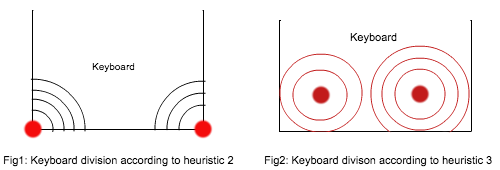
\includegraphics[scale=0.5]{heuristics}
\end{figure}

By defining this new feature (in different ways), we hope to enhance the ratio of error detection, especially for substitution. Weka algorithms will be implemented by learning decision trees to detect the errors.

\section{Evaluation}
Our evaluation will be done in a similar way to Clawson et al. We will use leave-one-out cross-validation to generate training and testing tests. Clawson et al used sliced the data set across various dimensions (user expertise, keyboards, visibility conditions and corpora) to test how well their algorithm generalizes. We will follow the same procedure.  Four data sets were collected for training and testing: Dell complete, Dell expert, Targus complete, and blind to test the validity of these features.

For each slice, we will look at the following for every type of error mentioned above (roll-on, roll-off, key repeat, and row substitution):
\begin{itemize}
\item Average possible corrections
\item Average corrections detected
\item Average wrong corrections
\end{itemize}

F-measure is not a good evaluator in this case, since a wrong correction constitutes a highly negative user experience, and hence cannot be weighted the same as a missed correction.  
We will also look specifically at off-by-one errors as they constitute a large percentage of the total errors.

We expect our algorithm to perform better than Automatic Whiteout++ on row substitution errors (since that is what our modified algorithm targets), specifically by reducing the average number of wrong corrections.

\section{Discussion}


\bibliographystyle{plain}
\bibliography{main}

\end{document}